\documentclass[tikz,border=0mm]{standalone}
\usepackage[T1]{fontenc}
\usepackage{lmodern,amsmath,amssymb}
\usetikzlibrary{arrows.meta}

\definecolor{Ink}{HTML}{173047}
\definecolor{Navy}{HTML}{17486F}
\definecolor{Slate}{HTML}{526D80}
\definecolor{Border}{HTML}{A4B6C2}
\definecolor{Light}{HTML}{F2F6F8}
\definecolor{Pale}{HTML}{E8F0F5}

\tikzset{
  stage/.style={draw=Border,fill=Light,line width=.55pt},
  result/.style={draw=Navy,fill=Pale,line width=.65pt},
  heading/.style={anchor=west,inner sep=0pt,font=\sffamily\bfseries\fontsize{10.3}{12}\selectfont},
  copy/.style={anchor=west,inner sep=0pt,align=left},
  decision/.style={draw=Navy,fill=white,line width=.9pt},
  arrow/.style={draw=Navy,line width=.7pt,-{Stealth[length=1.9mm,width=1.32mm]}},
  branch label/.style={anchor=west,inner sep=0pt,text=Slate,font=\sffamily\bfseries\fontsize{9.1}{11}\selectfont}
}

\begin{document}
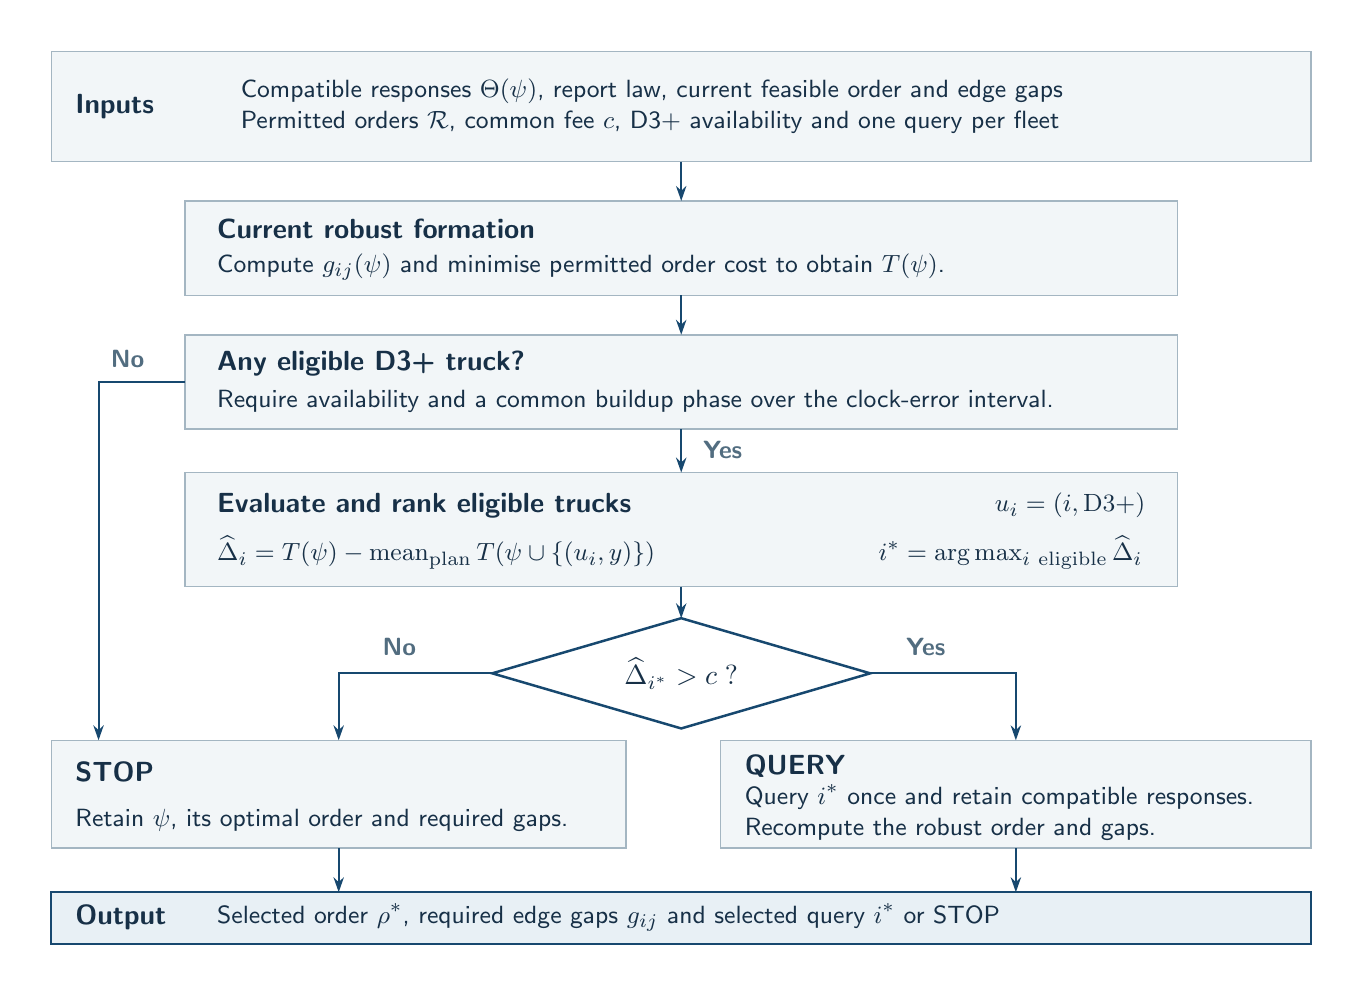
\begin{tikzpicture}[x=1mm,y=1mm,text=Ink,font=\sffamily\fontsize{9.3}{11.3}\selectfont]
\path[use as bounding box] (0,0) rectangle (166,118);
\fill[white] (0,0) rectangle (166,118);

% Inputs and the stop-now reference, computed on the same formation set.
\draw[stage] (3,101) rectangle (163,115);
\node[heading] at (6,108) {Inputs};
\node[copy] at (27,108) {Compatible responses \(\Theta(\psi)\), report law, current feasible order and edge gaps\\
  Permitted orders \(\mathcal R\), common fee \(c\), D3+ availability and one query per fleet};

\draw[stage] (20,84) rectangle (146,96);
\node[heading] at (24,92.4) {Current robust formation};
\node[copy] at (24,87.6) {Compute \(g_{ij}(\psi)\) and minimise permitted order cost to obtain \(T(\psi)\).};
\draw[arrow] (83,101) -- (83,96);

% Phase eligibility is checked before evaluating candidate gains.
\draw[stage] (20,67) rectangle (146,79);
\node[heading] at (24,75.4) {Any eligible D3+ truck?};
\node[copy] at (24,70.6) {Require availability and a common buildup phase over the clock-error interval.};
\draw[arrow] (83,84) -- (83,79);

\draw[stage] (20,47) rectangle (146,61.5);
\node[heading] at (24,57.3) {Evaluate and rank eligible trucks};
\node[anchor=east,inner sep=0pt] at (142,57.3) {\(u_i=(i,\mathrm{D3+})\)};
\node[copy] at (24,51.3) {\(\widehat\Delta_i=T(\psi)-\operatorname{mean}_{\mathrm{plan}}T(\psi\cup\{(u_i,y)\})\)};
\node[copy] at (108,51.3) {\(i^*=\arg\max_{i\ \mathrm{eligible}}\widehat\Delta_i\)};
\draw[arrow] (83,67) -- (83,61.5);
\node[branch label] at (85.7,64.4) {Yes};

% The score is gross. A tie with the common fee takes the STOP branch.
\path[decision] (83,43) -- (107,36) -- (83,29) -- (59,36) -- cycle;
\node[font=\sffamily\bfseries\fontsize{10.3}{12}\selectfont,inner sep=0pt]
  at (83,36) {\(\widehat{\Delta}_{i^*}>c\;?\)};
\draw[arrow] (83,47) -- (83,43);

\draw[stage] (3,13.8) rectangle (76,27.5);
\node[heading] at (6,23.5) {STOP};
\node[copy] at (6,17.4) {Retain \(\psi\), its optimal order and required gaps.};
\draw[arrow] (20,73) -- (9,73) -- (9,27.5);
\node[branch label] at (10.5,76) {No};
\draw[arrow] (59,36) -- (39.5,36) -- (39.5,27.5);
\node[branch label] at (45,39.4) {No};

\draw[stage] (88,13.8) rectangle (163,27.5);
\node[heading] at (91,24.2) {QUERY};
\node[copy] at (91,18.35) {Query \(i^*\) once and retain compatible responses.\\
  Recompute the robust order and gaps.};
\draw[arrow] (107,36) -- (125.5,36) -- (125.5,27.5);
\node[branch label] at (111.5,39.4) {Yes};

% Both terminal branches report through the same output block.
\draw[result] (3,1.6) rectangle (163,8.2);
\node[heading] at (6,5) {Output};
\node[copy] at (24,5) {Selected order \(\rho^*\), required edge gaps \(g_{ij}\) and selected query \(i^*\) or STOP};
\draw[arrow] (39.5,13.8) -- (39.5,8.2);
\draw[arrow] (125.5,13.8) -- (125.5,8.2);
\end{tikzpicture}
\end{document}
